\documentclass[tikz,border=10pt]{standalone}
\begin{document}
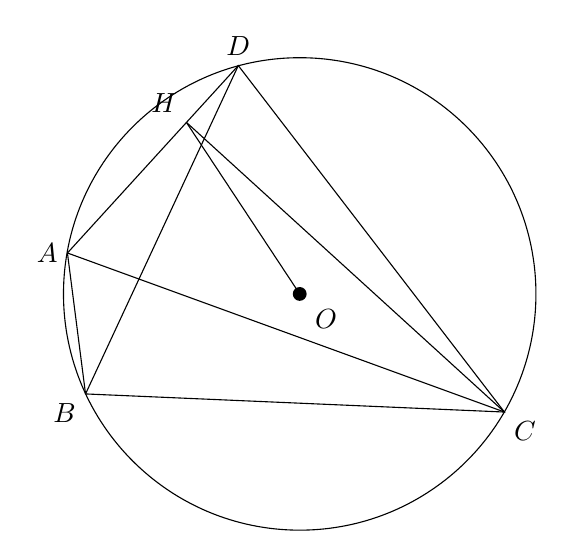
\begin{tikzpicture}[scale=1]
  \coordinate (O) at (0,0);
  \coordinate (A) at (-2.95,0.52);
  \coordinate (B) at (-2.72,-1.27);
  \coordinate (C) at (2.60,-1.50);
  \coordinate (D) at (-0.78,2.90);
  \coordinate (H) at (-1.44,2.18);

  \draw (O) circle (3);
  \draw (A) -- (B) -- (C) -- (D) -- cycle;
  \draw (A) -- (C);
  \draw (B) -- (D);
  \draw (H) -- (C);
  \draw (O) -- (H);
  \fill (O) circle (2.5pt);

  \node[above] at (D) {$D$};
  \node[left] at (A) {$A$};
  \node[below left] at (B) {$B$};
  \node[below right] at (C) {$C$};
  \node[above left] at (H) {$H$};
  \node[below right=2pt] at (O) {$O$};
\end{tikzpicture}
\end{document}
